\pagestyle{empty}
\tikzstyle{every picture}+=[remember picture]
\everymath{\displaystyle}
\begin{figure}[!ht]
\centering
\scalebox{.8}{

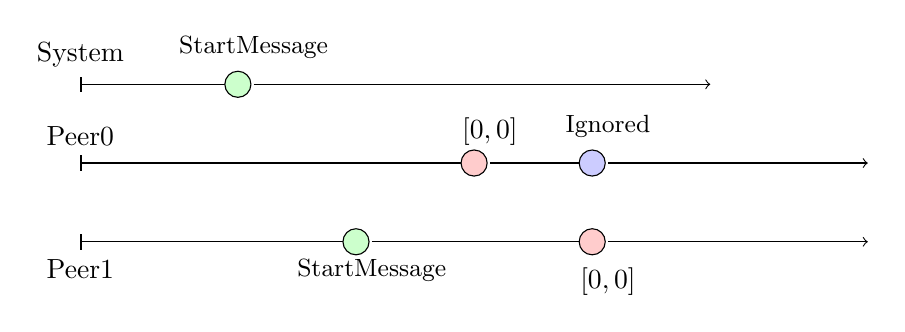
\begin{tikzpicture}

% SYSTEM TIMELINE
\draw[|-] (0,2) node[above=1mm]{System} -- (2,2) node{\tikz[baseline]{
	\node[fill=green!20,draw,circle] (sm){};
}};
\draw[->] (2.2,2) node[above=2mm]{\small{StartMessage}} -- (8,2) {};

% PEER 0
\draw[|-] (0,1) node[above=1mm]{Peer0} -- (5,1) node{\tikz[baseline]{
	\node[fill=red!20,draw,circle] (f0){};
}};
\draw[-] (5.2,1) node[above=1mm]{$[0,0]$} -- (6.5,1) node{\tikz[baseline]{
	\node[fill=blue!20,draw,circle] (f1){};
}};
\draw[->] (6.7,1) node[above=2mm]{\small{Ignored}} -- (10,1) node[below=1mm]{};

% PEER 1
\draw[|-] (0,0) node[below=1mm]{Peer1} -- (3.5,0) node{\tikz[baseline]{
	\node[fill=green!20,draw,circle] (e0){};
}};
\draw[-] (3.7,0) node[below=1mm]{\small{StartMessage}} -- (6.5,0) node{\tikz[baseline]{
	\node[fill=red!20,draw,circle] (e1){};
}};
\draw[->] (6.7,0) node[below=2mm]{$[0,0]$} -- (10,0) node[below=1mm]{};

\end{tikzpicture}

\begin{tikzpicture}[overlay]
    \path[->] (sm) edge [out=-90, in=135] (e0);
    \path[->] (sm) edge [out=-45, in=135] (f1);
    \path[->] (e0) edge [out=45, in=-135] (f0);
    \path[->] (f0) edge [out=-45, in=135] (e1);
\end{tikzpicture}

}

  \caption{An issue overcomed in our asyncronous simulation.}
\end{figure}
